\subsubsection{Rappel: Méthode d'intégration des fonctions de plusieurs variables}
\lecture{27}{2025-05-26}{Dernier cours???}{}


\begin{parag}{Théorème de Fubini $\implies$ changement d'ordre d'intégration}
   \begin{center}
       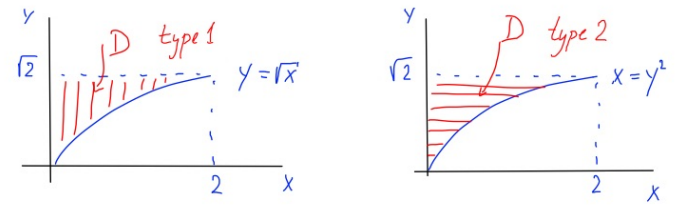
\includegraphics[scale=0.8]{12025-05-26.png}
   \end{center}
   Qui nous donne:
   \begin{align*} 
       \int_0^2dx\int_{\sqrt{x}}^{\sqrt{2}}f\left(x, y\right) dy =  \int_{0}^{\sqrt{2}}dy\int_0^{y^2}f\left(x, y\right)dx
   \end{align*}
\end{parag}
\begin{parag}{L'additivité de l'intégrale $\implies$ Division du domaine d'intégration}
    \begin{center}
        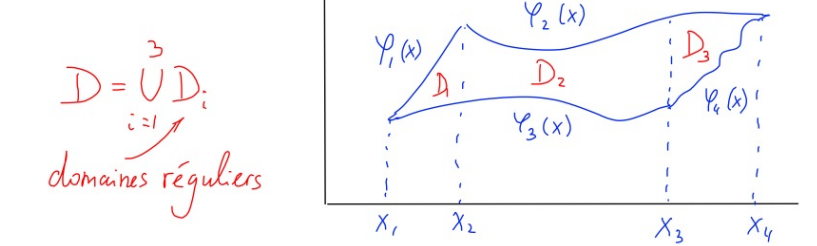
\includegraphics[scale=0.8]{22025-05-26.png}
    \end{center}
    Il faut diviser le domaine en réunion et utiliser l'additivité de l'intégrale.
    
    
\end{parag}
\begin{parag}{Changement de variable}
    
    \begin{theoreme}
    Soit $E \subset \mathbb{R}^{n} $ un sous-ensemble, $\overline{E}$ est compact, $\psi: E \to \mathbb{R}^{n}$ telle que $\psi \in C^1\left(E\right)$, et $\psi: E \to \psi\left(E\right) = D$ bijective. Soit $f : \overline{D}  = \overline{\psi\left(E\right)} \to \mathbb{R}$ un fonction continue. Alors:
    \begin{align*} \int_D f\left(\overline{x}\right) =  \int_E f\left(\psi\overline{u}\right)\left|\det J_{\psi\left(\overline{u}\right)}\right|d\overline{u} \end{align*}
    \end{theoreme}
        \begin{center}
            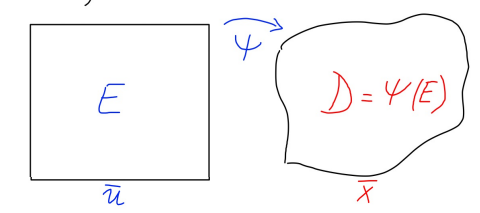
\includegraphics[scale=0.8]{32025-05-26.png}
        \end{center}
\end{parag}
\begin{parag}{Coordonnées sphérique}
    \begin{align*} 
        G\left(r, \theta, \phi\right) =  
        \begin{cases}
            x =  r \sin \theta \cos \phi\\
            y = r \sin \theta \sin \phi\\
            z =  r \cos \theta
        \end{cases}
    \end{align*}
    \begin{center}
        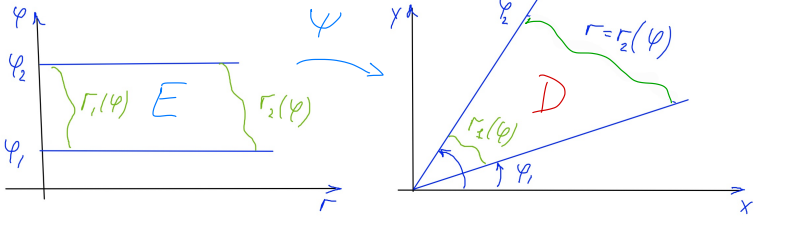
\includegraphics[scale=0.6]{42025-05-26.png}
    \end{center}
    \begin{align*} \left|\det J_{G\left(r, \theta, \phi\right)}\right| = r^2\sin\theta \end{align*}
\end{parag}
\begin{parag}{Exemple}
    Le volume d'un ellipsoide $\left\{\left(x, y, z\right) \in \mathbb{R}^{3}: \frac{x^2}{a^2} + \frac{y^2}{b^2} + \frac{z^2}{c^2} \leq 1\right\}$.
    On pose le changement de variable:
    \begin{align*} 
        \begin{cases}
            x =  au\\
            y = bv\\
            z = cw
            \end{cases} &\implies \left\{\left(u, v, w\right)\in \mathbb{R}^{3}: u^2 + v^2 + w^2 \leq 1\right\} \implies J_{H\left(u, v, w\right)} = \begin{pmatrix} a & 0 & 0 \\ 0 & b & 0 \\ 0 & 0 & c \end{pmatrix} \\
                        &\implies \left|\det J_H\right| = \left|abc\right| 
    \end{align*}
    \begin{center}
        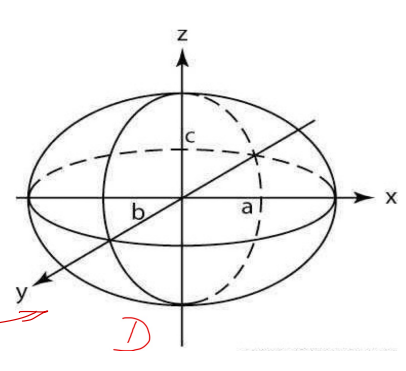
\includegraphics[scale=0.7]{62025-05-26.png}
    \end{center}
    
    Donc ici on en premier lieu, le changement de variable polaire (on passe de l'ellipsoide à une sphère) et ensuite de la sphère à un pavé:
    \begin{align*} 
        J_{H \mathring G} = J_{H\left(G\right)} \cdot  J_G = \left| \underbrace{\det J_{H\left(G\right)}}_{abc}\right| \cdot  \left|\underbrace{\det J_G}_{r^2 \sin \theta}\right| = abcr^2\sin\theta
    \end{align*}
    On a donc notre volume:
    \begin{align*}
        V =  \int_0^{2\pi}d\phi \int_0^\pi d \theta \int_0^1 abcr^2\sin\theta dr =  abc\int_0^{2\pi} d \phi \int_0^\pi \sin \theta d \theta \int_0^1 r^2 dr =  abc \frac{4}{3}\pi
    \end{align*}
\end{parag}
\begin{parag}{Coordonnées cylindriques}
    \begin{align*} 
    G\left(r, \theta, z\right) =     \begin{cases}
            x =  r \cos\phi\\
            y =  r \sin \phi\\
            z =  z
        \end{cases}
    \end{align*}
    On a donc notre fonction $G: [0, \infty[ \times [ 0, 2\pi[ \times \mathbb{R} \to \mathbb{R}^{3}  $, Je passe les details pour la jacobienne mais son déterminant est donnée par:
    \begin{align*} \det J_{G\left(r, \phi, z\right)} =  r \end{align*}
    \begin{center}
        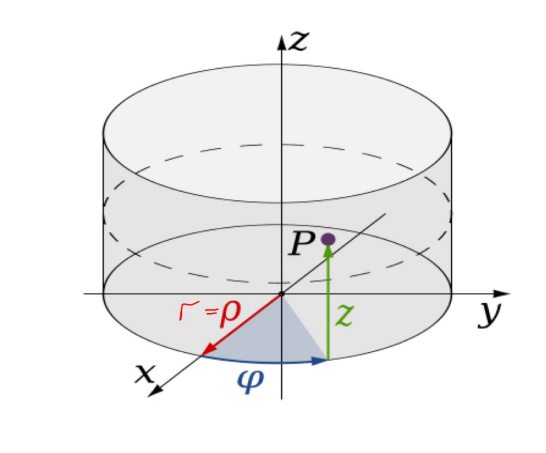
\includegraphics[scale=0.4]{72025-05-26.png}
    \end{center}
    
\end{parag}
\begin{parag}{Exemple}
    Trouver le volume du domaine $D$ avec les frontières:
    \begin{align*} 
        \begin{cases}
            x^2 + y^2 + z^2 =  2za, a > 0\\
            x^2 + y^2 =  z^2
        \end{cases}
    \end{align*}
    Qui contient $\left(0, 0, a\right)$. Donc ici comme on a des $x^2 + y^2$ mais dans $\mathbb{R}^{3}$ (sans le $+ z^2$) les coordonnés cylindrique sont utiles:
    \begin{align*} 
        \begin{cases}
            r^2 + z^2 - 2za = r^2 + z^2 - 2za + a^2 = a^2\\
            r^2 =  z^2
        \end{cases} \implies 
        \begin{cases}
            r^2 + \left(z-a\right)^2 =  a^2\\
            r = z, z \geq 0\\
            r =  -z, z \leq 0
        \end{cases}
    \end{align*}
    On a ici donc une sphère de rayon $a$ qui est centré en $\left(0, 0, a\right)$. Pour ce qui est de la deuxième équation, comme $r = z$, on a le rayon du cercle qui est égal à la hauteur, plus la hauteur plus le rayon du cercle augment (on parle pas de la sphère ici). Est donc on a un \important{cône}.\\
    On cherche donc l'intersection qui se trouve en $r = z$:
    \begin{align*} 
        a^2 &= r^2 + \left(r-a\right)^2 \\
           0 &=2r^2 + -2ra\\
             &= 2r\left(r-a\right) \implies r = a= z
    \end{align*}
    On a ici donc le cercle de rayon $a$ dans le plan $a = z$.\\
    On a donc notre volume qui se calcule avec la somme d'un demi sphère de rayon $a$ et d'un cône $r = z$ coupé par $0 < z < a$.\\
    Donc la démi sphère est donné par:
    \begin{align*} \frac{1}{2}\frac{4}{3}\pi a^3 =  \frac{2}{3}\pi a^3 \end{align*}
    On cherche donc maintenant le volume du cône (qui a donc un angle de $\frac{\pi}{4}$ (vu qu'on a $z = r$) et une hauteur de $a$):
    Si on écrit l'ensemble:
    \begin{align*} 
        D =  \left\{0 < z < a, 0 < \phi < 2\pi, 0 < r < z\right\}
    \end{align*}
    \begin{align*} 
        V &= \int_0^{2\pi}d\phi \int_0^a dz \int_0^z r dr = 2\pi \int_0^a \left(\frac{1}{2}r^2\mid_0^z\right)dz\\
          &= \pi \int_0^a z^2 dz\\
          &= \frac{1}{3}\pi z^3\mid_0^a = \frac{1}{3}\pi a^3
    \end{align*}
    On a donc le volume total:
    \begin{align*} V = \frac{2}{3}\pi a^3 + \frac{1}{3}\pi a^3 =  \pi a^3 \end{align*}
\end{parag}
\begin{parag}{Géométrique de changement de variables}
   \begin{framedremark}
        Dans le changement de variables sphériques et cylindriques, une coordonnée cartesienne est de la forme spéciale \important{$z$}. Mais selon la géométrique du domaine et la fonction donnée, on peut choisir une autre coordonnée cartesienne d'avoir cette forme spéciale, par exemple $y$
   \end{framedremark} 
   \begin{center}
       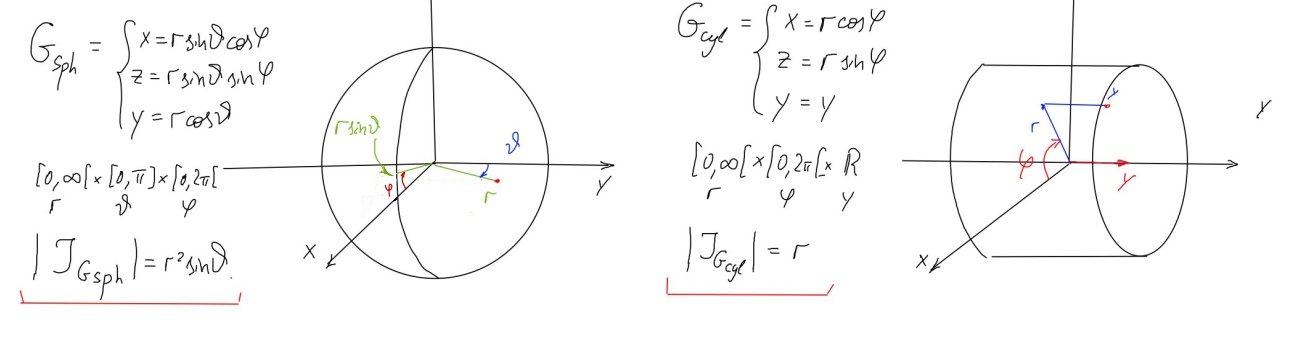
\includegraphics[scale=0.6]{82025-05-26.png}
   \end{center}
\end{parag}


\begin{parag}{Exemple}
    \begin{align*} 
        \int\int\int_E e^y dxdydz, \; \; E = \left\{\left(x, y, z\right) \in \mathbb{R}^{3}: x^2 +z^2 \leq 4, -\sqrt{x^2 + z^2} < y < \sqrt{x^2 + z^2}\right\}
    \end{align*}
   On a donc avec le changement de coordonnées cylindrique:
   \begin{align*} 
   \begin{cases}
       x =  r\cos \phi\\
       y = r\sin \phi\\
       z = z
   \end{cases}
   \end{align*}
   On a donc notre ensemble qui change:
   \begin{align*} 
       E =  \left\{\left(r, \phi, z\right): 0 < \phi < 2\pi, 0 < r < 2, -r < y < r^2\right\}
   \end{align*}
   Il nous reste plus qu'à intégrer (avec le déterminant de la jacobienne):
   \begin{align*} 
       \int_0^{2\pi}d \phi \int_0^2 dr \int_{-r}^{r^2}e^y \cdot  r dy
   \end{align*}
\end{parag}
\chapter{Fin du cours, Révision}

\section{Intégrale}
\begin{parag}{(1)}
    \begin{align*} 
        \int\int_D \arcsin \left(\frac{y}{\sqrt{x^2 + y^2}}\right)dxdy \\
        D = \left\{\left(x, y\right) \in \mathbb{R}^{2}: x \geq 0, y \leq 0, 1 \leq x^2 + y^2 \leq 9\right\}
    \end{align*}
    On voit ici qu'on a deux cercle (plus grand que $1$ et plus petit que $9$) et qu'on prends donc dans un seul cadran (celui ou $x \geq 0$ et $y \leq 0$.\\
    On va utiliser les coordonnées polaires: $D =  \left\{\left(r, \phi\right): -\frac{\pi}{2} < \phi < 0, 1 < r < 3\right\}$  on obtient donc:
    \begin{align*} 
        \int_{-\frac{\pi}{2}}^{0}d \phi \int_1^3 \arcsin\left(\frac{r \sin\phi}{r}\right)\cdot r dr &= \int_{-\frac{\pi}{2}}^0d \phi \int_1^3 \phi r dr\\
                                                                                                    &= \frac{1}{2}\phi^2\mit_{-\frac{\pi}{2}}^0 \cdot  \frac{1}{2}r^2\mid_1^3 = -\frac{1}{2}\pi^2
    \end{align*}
\end{parag}
\begin{parag}{(2)}
    \begin{align*} \int\int\int_V z^2 dxdydz \end{align*}
    Avec comme domaine:
    \begin{align*} V =  \left\{\left(x, y, z\right): x <y, x^2 + y^2 < 4, 0 < z < \left(x^2 + y^2\right)^{\frac{1}{4}}\right\} \end{align*}
    Donc on a ici un cercle centré en $\left(0, 0, 0\right)$ de rayon $2$ coupé par la droite $x =  y$ et nous prenons ce qu'il y a au dessus de cette droite, le demi cercle au dessus de la droite $x = y$.\\
    Pour ce qui est du $z$ c'est pas très clair donc on préfère ``l'ignorer'' pour l'instant.\\
    Donc par changement de variable on a:
    \begin{align*} 
        V =  \left\{\left(r, \phi, z\right): \frac{\pi}{4} < \phi < \frac{5\pi}{4}, 0 < r < 2, 0 < z < \sqrt{r}\right\}
    \end{align*}
    On a donc si on réécrit l'intégrale:
    \begin{align*} 
        \int\int\int_V z^2 dxdydz &= \int_{\frac{\pi}{4}}^{\frac{5\pi}{4}}d\phi \int_0^2 dr \int_0^{\sqrt{r}}z^2 r dz\\
                                  &= \phi \mid_{\frac{\pi}{4}}^{\frac{5\pi}{4}} \cdot  \int_0^2 r \frac{1}{3}z^3 \mid_0^{\sqrt{r}}dr\\
                                  &= \pi \cdot  \frac{1}{3}\int_0^2 r^{\frac{5}{3}}dr = \frac{\pi}{3}\cdot  \frac{2}{7} \cdot  r^{\frac{7}{2}}\mid_0^2\\
                                  &= \frac{16\pi}{21}\sqrt{2}
    \end{align*}
\end{parag}
\begin{parag}{(3)}
    \begin{align*} \int\int\int_D \end{align*}
    Avec le domaine 
    \begin{align*} 
        D =  \left\{\left(x, y\right)\in \mathbb{R}^{2}: -1 \leq y \leq 1, y^2 \leq x \leq 1\right\}
    \end{align*}
    On a donc ici la fonction $y =  x^2$ renvérsé (sur le côté) de $x =  y^2$ et $x =  \left(-y\right)^2$:
    \begin{align*} 
        \int_{-1}^1 dy \int_{y^2}^1 \sin y \cos x dx &=\int_{-1}^1dy\left(\sin y\left( \sin 1 - \sin\left(y^2\right)\right)\right)
    \end{align*}
    Néanmoins la fonction $\sin\left(y^2\right)$ n'a pas de primitive de fonction usuelle donc on va simplement essayer avec un autre type. Donc ici ça sera le $x$ qui varie entre deux nombre et le $y$ qui lui entre des fonctions de $x$:
    \begin{align*} 
        D =  \left\{\left(x, y \right) \in \mathbb{R}^{2}: 0 < x < 1, -\sqrt{x} < y <\sqrt{x}\right\}
    \end{align*}
    Si on réécrit donc notre intégrale on a:
    \begin{align*} 
        \int_0^1 dx \int_{-\sqrt{x}}^{\sqrt{x}}\sin y \cos x dx &= \int_0^1dx \left(\cos x \left(-\cos y\right)\right)\mid_{-\sqrt{x}}^{\sqrt{x}}\\
                                                                &= \int_0^1 \cos x \left(-\cos \sqrt{x} + \cos \left(-\sqrt{x}\right)\right)dx\\
                                                                &= 0
    \end{align*}
    Ici on voit ici qu'on a $f\left(x, y\right) =  \sin y \cos x$ mais on voit que cette dernière est pair: $f\left(x, -y\right) = \sin$ (pas eu le temps mais ducoup ca faisait 0)
\end{parag}
\begin{parag}{Question 23}
    Soit $D =  \left\{\left(x, y\right)\in \mathbb{R}^{2}: x \geq -1, \left|y\right| \leq 1 - x\right\}$. On demande la forme de cette ensemble.\\
    \begin{subparag}{Réponse}
        Ici on peut remarque deux truc important, on a la ``réciproque'' (pas formellement mais à peu près) de la fonction $f\left(x\right) =  \left|x\right|$. Ensuite on a fonc les max se trouve $ x =  -1$ et si on évalue pour $y$: $\left|y\right| = 1 - - 1$ ce qui nous donne donc $\left|y\right|= 2 \implies  y =\pm 2$. donc on à un triangle avec les point $\left(-1, \pm 2\right)$. Ensuite on a donc le maximum pour $x =  1$ et donc $y =  0$. 
    \end{subparag}
\end{parag}

\begin{parag}{Question 24}
    L'intégrale $\int_{\frac{\pi}{4}}^{\frac{\pi}{2}}d \phi \int_o^{\frac{1}{\sin \phi}}r dr$ exprime l'aire d'un(e):
    \begin{itemize}
        \item Secteur circulaire
        \item Triangle
        \item Rectangle
        \item Tranche d'un cercle
    \end{itemize}
    \begin{subparag}{Réponse}
        Donc déjà on a des coordonnés polaires avec donc $D = \left\{\left(\phi, r\right): \frac{\pi}{4} < \phi < \frac{\pi}{2}, 0 < r < \frac{1}{\sin \phi}\right\}$. On a donc $0 < r < \frac{1}{\sin \phi}$ ce qui est une droite
    \end{subparag}
\end{parag}

